\section{Introduction}\label{s:intro}

A lower bound for a van der Waerden number is witnessed by a colouring that
avoids long monochromatic arithmetic progressions. At the sizes considered
here, such a colouring contains tens of billions of positions. Its description,
however, need not be comparably large. In Rabung's power-residue construction,
a triple of integers $(p,r,k)$ determines the finite conditions from which the
colouring and its lower bound follow. The computational problem is to find a
useful triple; the mathematical problem is to verify those conditions and to
place the bound among the consequences of earlier constructions.

For integers $r\ge2$ and $k\ge3$, let $W(r,k)$ be the least $N$ such that
every $r$-colouring of $\{1,\dots,N\}$ contains a monochromatic arithmetic
progression of length $k$. We put colours first. Monroe~\cite{Monroe2026}
uses the reverse convention $W(k,r)$; Fox and Hunter~\cite{FoxHunter2026}
write $w(k;r)$.

\subsection{Numerical results and their scope}

We obtain three primitive three-colour Rabung certificates, at lengths
$17$, $18$ and $19$. They give nine direct inequalities for $17\le k\le25$;
the final six follow from the length-19 certificate by a fixed-prime
monotonicity lemma. In particular,
\[
 W(3,17)>31\,385\,622\,833,
\]
using $p=1\,961\,601\,427$. This is a factor $2.02$ above the earlier
$15\,509\,557\,937$ listed by Monroe. The five inequalities for
$17\le k\le21$ improve the prior comparators identified in the source review
updated on 26~September~2026; Table~\ref{tab:priority} gives their values.

A new direct certificate need not give a better general bound. For
$22\le k\le25$, our certificates improve the Rabung rows located in the
review, but stronger bounds already follow from other constructions. A
stronger published statement of Landman and Robertson has an unresolved
proof status in our audit. We display its consequences separately and include
it among prior comparators: the five improvements at lengths $17$--$21$
remain, whereas it dominates the admitted table at lengths $24$--$28$.
This is a comparison with a dated, explicit corpus, not an assertion of
exhaustive global priority.

We also recheck four two-colour certificates from the archived second phase of
Monroe's distributed project~\cite{MonroePhase2Archive}, retaining the credit
of that project and its volunteers. Together with the nine three-colour rows,
they form the thirteen inequalities of Theorem~\ref{thm:certified-rabung}.
Only seven triples are primitive; the archived rechecks deliberately retain
the redundant consequences.

\subsection{From a short certificate to a finite comparison}

Multiplication by a nonzero residue permutes the colour classes of a
power-residue colouring. After such a dilation, an arithmetic progression
becomes a consecutive string. Rabung's theorem reduces the large-colouring
problem to a run-length test and a condition at the multiples of
$p$~\cite{rabung1979}. A qualifying prime gives $W(r,k)>(k-1)p+1$.
We prove the equivalence of the implemented boundary test with the published
criterion and provide a stand-alone CPU checker whose source and arithmetic
are separate from the GPU search. The small example in
Section~\ref{ss:criterion} illustrates the reduction before the proof.

\begin{figure}[htbp]
\centering
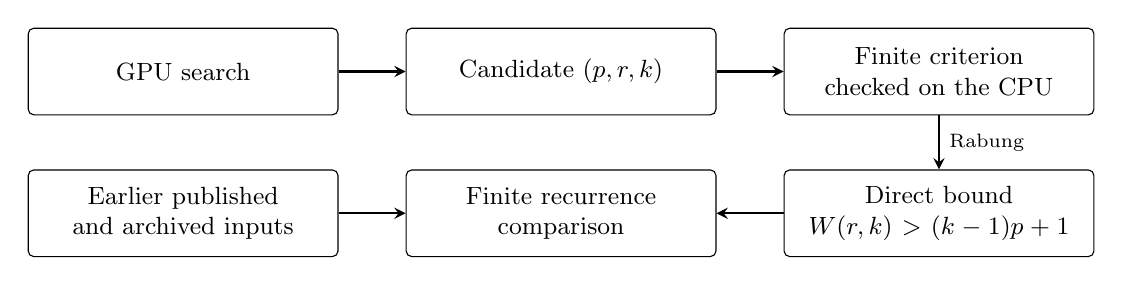
\begin{tikzpicture}[>=stealth,box/.style={draw,rounded corners=2pt,
  align=center,font=\small,minimum height=11mm,text width=3.7cm},
  edge/.style={->,thick}]
\node[box] (search) at (0,0) {GPU search};
\node[box] (triple) at (4.8,0) {Candidate $(p,r,k)$};
\node[box] (check) at (9.6,0) {Finite criterion\\checked on the CPU};
\node[box] (prior) at (0,-1.8) {Earlier published\\and archived inputs};
\node[box] (closure) at (4.8,-1.8) {Finite recurrence\\comparison};
\node[box] (bound) at (9.6,-1.8) {Direct bound\\$W(r,k)>(k-1)p+1$};
\draw[edge] (search)--(triple);
\draw[edge] (triple)--(check);
\draw[edge] (check)--node[right,font=\scriptsize]{Rabung}(bound);
\draw[edge] (bound)--(closure);
\draw[edge] (prior)--(closure);
\end{tikzpicture}
\caption{The two steps after discovery. The candidate can be checked without
replaying the search, and its bound is compared with consequences of earlier
inputs. Campaign coverage and the empirical intensity analysis are separate
from these pointwise implications.}
\label{fig:evidence-flow}
\end{figure}


Earlier bounds must then be compared under known recurrences. For example,
Blankenship, Cummings and Taranchuk~\cite[Theorem~2.1]{bct2018} prove
\begin{equation}\label{eq:bct-intro}
 W(r,k)>q\left(W\!\left(r-\left\lceil r/q\right\rceil,k\right)-1\right)
\end{equation}
for a prime $q\le k$. For three colours, an earlier strict bound
$W(2,k)>B$ gives $W(3,k)>q_kB$, where $q_k$ is the largest prime at most
$k$. This explains why a larger Rabung prime need not yield the strongest
general bound. Our finite comparison also includes length monotonicity and
the registered Xu operation~\cite{xu2013,Monroe2026}, with exact integers
and a provenance path for every retained value. No winning three-colour row
depends on Xu.

\subsection{Relation to earlier work}

Computational power-residue constructions and cyclic-zipper extensions have
been developed by Herwig, Heule, van Lambalgen and van Maaren~\cite{herwig2007},
Rabung and Lotts~\cite{rabunglotts2012}, Liang, Xu, Shao and
Xiu~\cite{liang2012}, and Monroe~\cite{Monroe2016v1,Monroe2017v4,Monroe2026}.
Publishing a prime together with checking code has antecedents in this
literature. Our contribution is the three new primitive certificates, their
separate verification, and their explicit comparison with consequences of
the identified prior inputs. Certification is not presented as a new principle.

Berlekamp's construction supplies a stronger admitted bound at length $24$,
inherited at length $25$~\cite{Berlekamp1968}. The stronger
Landman--Robertson statement requires the separate treatment just
described~\cite{LandmanRobertson2004,LandmanRobertson2014,Johannson2007}.
The recent superexponential three-colour result of Fox and
Hunter~\cite{FoxHunter2026} and the asymptotic two-colour bound
$w(k)\ge(1-o(1))k2^{k-1}$ of Campos, Fox and
Schildkraut~\cite{CamposFoxSchildkraut2026} address different asymptotic
questions. In the version-pinned sources examined, neither supplies a
stronger explicit finite entry for our window.
Gasarch and Haeupler's explicit family
$W(3,k)\ge3^{k-1}/(ek)$~\cite[Note~1.7(2)]{GasarchHaeupler2011} is retained
in the registry and is dominated there. Kozik and
Shabanov~\cite[Theorem~2 of the arXiv version]{KozikShabanov2014} give
$W(r,k)\ge\beta r^{k-1}$ for an absolute $\beta>0$; no finite improvement
from that theorem is asserted here. Hunter's exponential improvement begins
at five colours~\cite{Hunter2025} and does not change the three-colour table.

\subsection{Reading guide and evidence boundary}

Section~\ref{s:bounds} gives the numerical results and their comparison.
Section~\ref{s:method} explains the construction, proves the boundary-test
equivalence and describes the checker. Section~\ref{s:campaign} explains
the discovery and verification protocol. The search covered
$[9.7\times10^8,2\times10^9)$ in $515$ chunks; its coverage evidence has a
separate role from the validity of any one certificate.

A reader interested in the inequalities can read the results and the
criterion proof first. The witness is short, but a complete recheck still
visits a linear number of residues and evaluates their colours; checking the
identities of the retained archive is a separate, much lighter operation. The source catalogue, campaign audit and execution
identities remain available in the appendices and accompanying package.
Appendices~\ref{s:prereg}--\ref{s:densitydiagnostics} compare three fixed
search-intensity forecasts on one run-valid $(3,17)$ trajectory. That empirical
comparison neither proves a density law nor enters the lower-bound proof.
No independently administered external replication has been performed; the
preserved local computations and their limits are stated throughout.
